\documentclass[12pt,twoside]{report}

\usepackage[utf8]{inputenc}
\usepackage[spanish]{babel}

\usepackage{amsmath}
\usepackage{amsfonts}
\usepackage{amssymb}

\usepackage{setspace}

\usepackage{enumitem}

\usepackage[normalem]{ulem}

\usepackage[table,xcdraw]{xcolor}

\usepackage[export]{adjustbox}
\usepackage[official]{eurosym}
\usepackage{longtable}
%%%%%%%%%%%%%%%%%%%%%%%%%%%%%%%%%%%%%%%%%%%%%%%%%%%%%%%%%%%%%%%%%%%%%%%%%%%%%

% Definitions for the title page
\newcommand{\reporttitle}{
	Solicitud de Subvención\\
	y \\
	Memoria de Actividades 2014-15
}
\newcommand{\reportauthor}{Asociación Club de Robótica-Mecatrónica}



\setlength{\parskip}{\baselineskip}
\setlength{\parindent}{0pt}

\usepackage{hyperref}
\hypersetup{
    hyperindex, linktoc=page, breaklinks,
    pdfauthor=\reportauthor,pdftitle=\reporttitle
}
%%%%%%%%%%%%%%%%%%%%%%%%%%%%%%%%%%%%%%%%%%%%%%%%%%%%%%%%%%%%%%%%%%%%%%%%%%%%%

% load some definitions and default packages
%%%%%%%%%%%%%%%%%%%%%%%%%%%%%%%%%%%%%%%%%
% University Assignment Title Page 
% LaTeX Template
% Version 1.0 (27/12/12)
%
% This template has been downloaded from:
% http://www.LaTeXTemplates.com
%
% Original author:
% WikiBooks (http://en.wikibooks.org/wiki/LaTeX/Title_Creation)
%
% License:
% CC BY-NC-SA 3.0 (http://creativecommons.org/licenses/by-nc-sa/3.0/)
% 
%
%%%%%%%%%%%%%%%%%%%%%%%%%%%%%%%%%%%%%%%%%
%----------------------------------------------------------------------------------------
%	PACKAGES AND OTHER DOCUMENT CONFIGURATIONS
%----------------------------------------------------------------------------------------
%\usepackage[a4paper,left=2.8cm,right=2.8cm,vmargin=2.0cm,includeheadfoot]{geometry}
\usepackage[a4paper,left=3.5cm,right=2.1cm,vmargin=2.0cm,includeheadfoot]{geometry}

\usepackage{textpos}

\usepackage{tabularx,longtable,multirow,subfigure,caption}
\usepackage{fncylab} %formatting of labels
\usepackage{fancyhdr} % page layout
\usepackage{url} % URLs

\usepackage{amsmath}
\usepackage{graphicx}
\usepackage{dsfont}

\usepackage{array}
\usepackage{latexsym}



%%% Default fonts
\renewcommand*{\rmdefault}{bch}
\renewcommand*{\ttdefault}{cmtt}



%%% Default settings (page layout)
\setlength{\parindent}{0em}  % indentation of paragraph

\setlength{\headheight}{14.5pt}
\pagestyle{fancy}
\renewcommand{\chaptermark}[1]{\markboth{\chaptername\ \thechapter.\ #1}{}} 

\fancyfoot[EL,OR]{\sffamily\textbf{\thepage}}%Page no. in the left on odd pages and on right on even pages
\fancyfoot[OC,EC]{\sffamily }
\renewcommand{\headrulewidth}{0.1pt}
\renewcommand{\footrulewidth}{0.1pt}
\captionsetup{margin=10pt,font=small,labelfont=bf}


%--- chapter heading

\def\@makechapterhead#1{%
  \vspace*{10\p@}%
  {\parindent \z@ \raggedright \sffamily
    \interlinepenalty\@M
    \Huge\bfseries \thechapter \space\space #1\par\nobreak
    \vskip 30\p@
  }}

%---chapter heading for \chapter*  
\def\@makeschapterhead#1{%
  \vspace*{10\p@}%
  {\parindent \z@ \raggedright
    \sffamily
    \interlinepenalty\@M
    \Huge \bfseries  #1\par\nobreak
    \vskip 30\p@
  }}

\allowdisplaybreaks


\date{Diciembre de 2015}

\addto\captionsspanish{\renewcommand{\chaptername}{Parte}}

\begin{document}

\begin{titlepage}

\newcommand{\HRule}{\rule{\linewidth}{1mm}} % Defines a new command for the horizontal lines, change thickness here


%----------------------------------------------------------------------------------------
%	LOGO SECTION
%----------------------------------------------------------------------------------------


\includegraphics[width = 6cm]{fotos/logo-eps.png}
\hfill

\includegraphics[width = 6cm]{fotos/logo-uam.png}



\center % Center remainder of the page

%----------------------------------------------------------------------------------------
%	HEADING SECTIONS
%----------------------------------------------------------------------------------------

%\textsc{\Large Escuela Politécnica Superior}\\[0.1cm]
%\textsc{\Large Universidad Autónoma de Madrid}\\[0.5cm]
\vspace{1cm}

%----------------------------------------------------------------------------------------
%	TITLE SECTION
%----------------------------------------------------------------------------------------


\HRule \\[0.4cm]
\begin{spacing}{1.5}
{ \fontsize{0.8cm}{1em} \bfseries \reporttitle}\\ % Title of your document
\vspace{0.5cm}
{ \fontsize{0.7cm}{1em} \bfseries \reportauthor} \\
\end{spacing}
\HRule \\[1.5cm]



\includegraphics[width = 7cm]{fotos/logo_crm-192x192.png}

{\large Asociación Club de Robótica-Mecatrónica (CRM-UAM)} \\
Local B-111 -- Escuela Politécnica Superior

\vfill

\textsc{\Large Universidad Autónoma de Madrid}\\[0.5cm]

\vfill

%----------------------------------------------------------------------------------------
%	FOOTER & DATE SECTION
%----------------------------------------------------------------------------------------


\makeatletter
{ \Large \@date }
\vfill
\makeatother


\end{titlepage}

\clearpage{\pagestyle{empty}\cleardoublepage}


% page numbering etc.
\pagenumbering{roman}
\setcounter{page}{1}
\pagestyle{fancy}






\begin{spacing}{0.1}
\tableofcontents
\end{spacing}

\clearpage{\pagestyle{empty}\cleardoublepage}

\pagenumbering{arabic}
\setcounter{page}{1}

\fancyhead[LE,RO]{\slshape}
%\fancyhead[LE,RO]{\slshape \rightmark}
\fancyhead[LO,RE]{\slshape \leftmark}

%%%%%%%%%%%%%%%%%%%%%%%%%%%%%%%%%%%%


\chapter{Presupuesto para nuevas actividades}


\section{Renovación del taller del club de robótica}
\subsubsection{Introduccion}

\section{Proyectos de construcción propia}

\subsection{Adaptación del cuadricóptero para vuelo autónomo}
\subsubsection{Responsable de proyecto y equipo de trabajo}
Jaime y Rodrigo
\subsubsection{Descripción}
\subsubsection{Objetivos}
\subsubsection{Contenido}
\subsubsection{Previsión de desarrollo}
\subsubsection{Presupuesto}


\subsection{Construcción Fresadora Cyclone PCB}
\subsubsection{Responsable de proyecto y equipo de trabajo}
Carlos y Victor
\subsubsection{Descripción}
\subsubsection{Objetivos}
\subsubsection{Contenido}
\subsubsection{Previsión de desarrollo}
\subsubsection{Presupuesto}


\subsection{Contrucción de un Escáner 3D}
\subsubsection{Responsable de proyecto y equipo de trabajo}
Carlos y Víctor
\subsubsection{Descripción}
\subsubsection{Objetivos}
\subsubsection{Contenido}
\subsubsection{Previsión de desarrollo}
\subsubsection{Presupuesto}


\section{Organización de talleres formativos para alumnos de la Universidad}

\subsection{Taller: Introducción a las FPGAs}
\subsubsection{Responsable de proyecto y equipo de trabajo}
Carlos
\subsubsection{Descripción}
\subsubsection{Objetivos}
\subsubsection{Contenido}
\subsubsection{Previsión de desarrollo}
\subsubsection{Presupuesto}


\subsection{Taller: Diseño e Impresión 3D (Open Hardware)}
\subsubsection{Responsable de proyecto y equipo de trabajo}
Carlos y Victor
\subsubsection{Descripción}
Se trata de un taller de modelado 3D orientado a la robótica, daremos una introducción a los participantes del uso de la herramienta libre OpenSCAD para el diseño de piezas 3D. Además queremos realizar pequeños retos prácticos en los que los participantes puedan poner en práctica lo aprendido. También se dará una charla sobre impresión 3D y finalizaremos mostrando como utilizar la impresora 3D existente en el club imprimiendo los mejores trabajos realizados por los participantes.
\subsubsection{Objetivos}
Queremos fomentar el diseño de open hardware entre los estudiantes de la universidad.
\subsubsection{Contenido}
\subsubsection{Previsión de desarrollo}
\subsubsection{Presupuesto}



\subsection{Taller: Introducción a la robótica con Arduino}
\subsubsection{Responsable de proyecto y equipo de trabajo}
\subsubsection{Descripción}
Es habitual en el Club de Robótica realizar un taller prático de introducción a la robótica para los alumnos de la Escuela Politécnica Superior. Consideramos muy importante de cara al año que viene realizar este taller para dar a conocer el club a nuevos alumnos con interés en robótica pero sin conocimientos previos.
\begin{figure}[hbtp]
\centerline{
\includegraphics[width=0.33\linewidth]{fotos/2012_taller_arduino_pantallas.jpg} 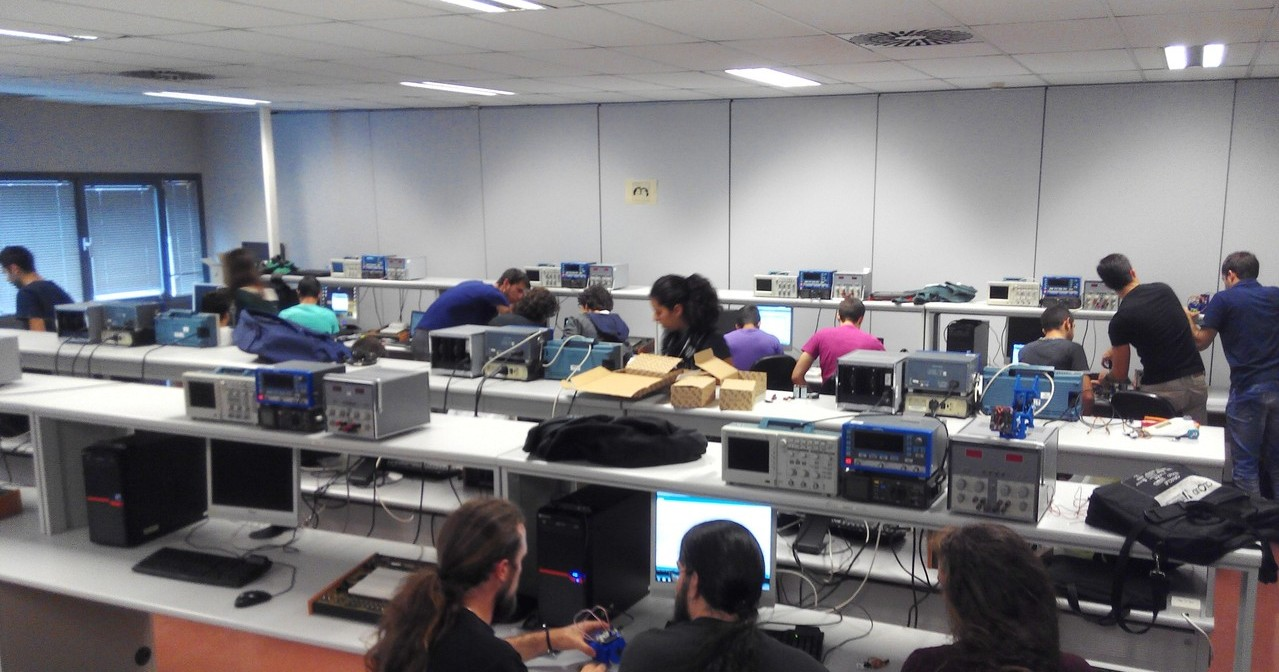
\includegraphics[width=0.4\linewidth]{fotos/fotoParticipantesArduparty.jpg} 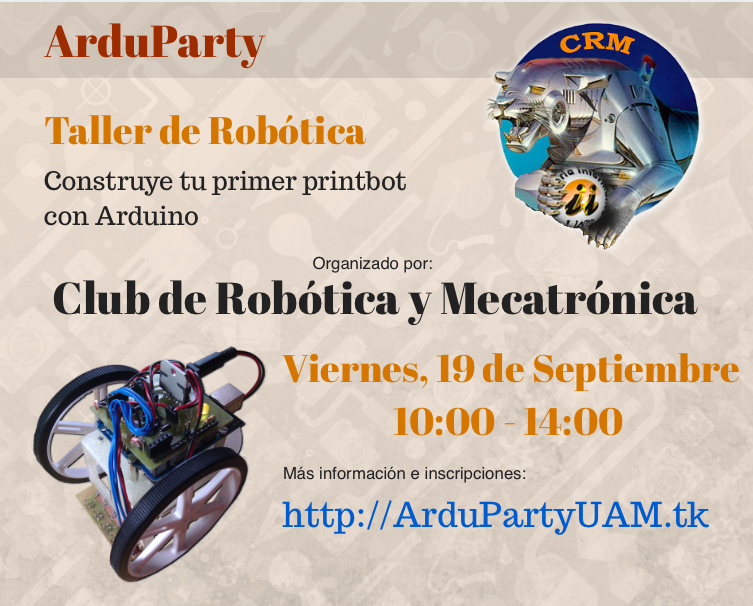
\includegraphics[width=0.33\linewidth]{fotos/2014_Cartel_ArduParty.png}}
\caption*{
Ediciones previas del taller.
}
\end{figure}

\subsubsection{Objetivos}
Seguir fomentado el conocimiento de la robótica entre los estudiantes de carreras técnicas. Dar a conocer nuestra asociación a estudiantes interesados y la nueva disponibilidad del taller del club para intenta fomentar que se creen nuevos grupos de trabajo autónomos dentro de la asociación.\\
Tenemos que seguir ofreciendo cada vez a más estudiante la posibilidad de realizar proyectos novedosos en el ámbito de la robótica y darles un pequeño empujón y respaldo necesario para llevarlos a cabo.\\
Acercar la plataforma Arduino, el diseño de Open Hardware y el diseño de estructuras 3D.
\subsubsection{Contenido}
El contenido del curso es fundamentalmente el mismo que el de la edición pasado, reutilizaremos los robots diseñados especificamente para esa edición basados en la plataforma Arduino. Los participantes tendran que realizar el montaje de sus kits y las conexiones electricas. \\
\begin{figure}[hbtp]
\centerline{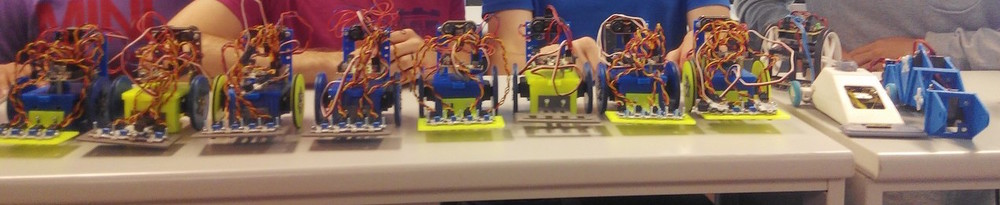
\includegraphics[width=1\linewidth]{fotos/robots_ArduParty.jpg}}
\caption*{
Robots ensamblados.
}
\end{figure}
Con el robot ya montado realizarmos diversas prácticas de programación y realizaremos interesantes retos guiando a los participantes en todo momento e introduciendoles de esta forma en la plataforma Arduino.\\
También profundizaremos en la comunicación entre Android y Arduino (Smartphone y Robot) programando una aplicación sencilla que nos permita controlar el robot desde el móvil.
\subsubsection{Previsión de desarrollo}
\subsubsection{Presupuesto}
Reutilizaremos los robots montados en la pasada edición del taller por lo que el presupuesto necesario es mínimo. \\
Para mejorar y suplir las deficiencias de la pasada edición necesitamos comprar baterías (pilas recargables) y cargadores para tener una mayor autonomía.\\
\begin{table}[htbp]
\centering\resizebox{16cm}{!} {
\begin{tabular}{|l|l|l|l|}
\hline
\multicolumn{1}{|c|}{\textbf{Producto}} & \multicolumn{1}{c|}{\textbf{Encale de compra}}                                   & \multicolumn{1}{c|}{\textbf{Precio Unitario}} & \multicolumn{1}{c|}{\textbf{Unidades}} \\ \hline
Pilas Recargables 9V                    & \scalebox{.8}{\href{http://es.rs-online.com/web/p/pilas-recargables-9-voltios/7033524/}{http://es.rs-online.com/web/p/pilas-recargables-9-voltios/7033524/}}              & 10,28\euro{}                                        & 8                                      \\ \hline
Cargador Pilas 9V                       & \scalebox{.8}{\href{http://es.rs-online.com/web/p/cargadores-de-pilas-aaa-aa-c-d-9- voltios/5177789/}{http://es.rs-online.com/web/p/cargadores-de-pilas-aaa-aa-c-d-9- voltios/5177789/}} & 15,10\euro{}                                        & 2                                      \\ \hline
\end{tabular}
}
\centering
\caption{presupuesto taller de introducción a la robótica}
\end{table}


\subsection{Taller: Sistemas embebidos. Raspberry Pi}
\subsubsection{Responsable de proyecto y equipo de trabajo}
\subsubsection{Descripción}
\subsubsection{Objetivos}
\subsubsection{Contenido}
\subsubsection{Previsión de desarrollo}
\subsubsection{Presupuesto}


\section{Organización de concursos internos y fomento de la robótica entre los estudiantes}


\section{Participación en eventos nacionales y representación de la UAM}

\section{Solicitud de subvención}








\chapter{Memoria del curso anterior}

\section{Talleres y proyectos internos}

\subsection{Construcción de un cuadrucóptero}

\subsection{Construcción de un robot para resolver laberintos}

\subsection{Uso de la impresora 3D por estudiantes}

\subsection{Re-organización del local para fomentar la participación}

\begin{itemize}
\item Actualización de la página web y creación de repositorio GitHub para el control de versiones
\item Limpieza del local (reciclado de equipos obsoletos que ocupaban espacio, mesas despejadas para facilitar la labor del equipo de limpieza)
\item Organización del material de los armarios y de las herramientas gracias a un panel de madera con ganchos.
\item Cada estudiante puede solicitar una caja de proyecto donde guardar todo el material que necesite. Dichas cajas están etiquetadas con su nombre y año, de este modo es posible organizar mejor el inventario disponible.
\end{itemize}

El nuevo enfoque del Club de Robótica es apoyar a cualquier miembro de la comunidad universitaria que quiera llevar a cabo proyectos relacionados con la robótica. Es decir, tanto estudiantes como profesores pueden inscribirse y así disponer de un espacio de trabajo agradable con herramientas de uso común (impresoras 3D, soldadores, sierras, alicates, destornilladores, etc) así como los materiales necesarios (cables, componentes, motores, baterías, etc).

Además disponemos de un foro donde nos ayudamos unos a otros, y periódicamente seguimos organizando actividades para fomentar la robótica entre los estudiantes.


\section{Participación en eventos nacionales}


\subsection{Concurso de resol. de laberintos en la OSHWDem (A Coruña)}


\subsection{Asistencia a la V jornada GMV de robótica (Tres Cantos)}


El 26 de Noviembre de 2015 asistimos desde el Club de Robótica al evento que tuvo lugar en la sede oficial de GMV, situada en Tres Cantos. Allí se realizaron demostraciones en directo de los robots Foxiris (para monitorización de plantas oil \& gas), MiR100 (un robot de exploración de tipo rover) y Aunav (un robot usado para la desactivación de explosivos)\footnote{Noticia en la web de GMV: \url{http://www.gmv.com/es/Empresa/Comunicacion/NotasDePrensa/2015/NP_017_VJornadaRobotica.html}}.

\begin{figure}[hbtp]
\centerline{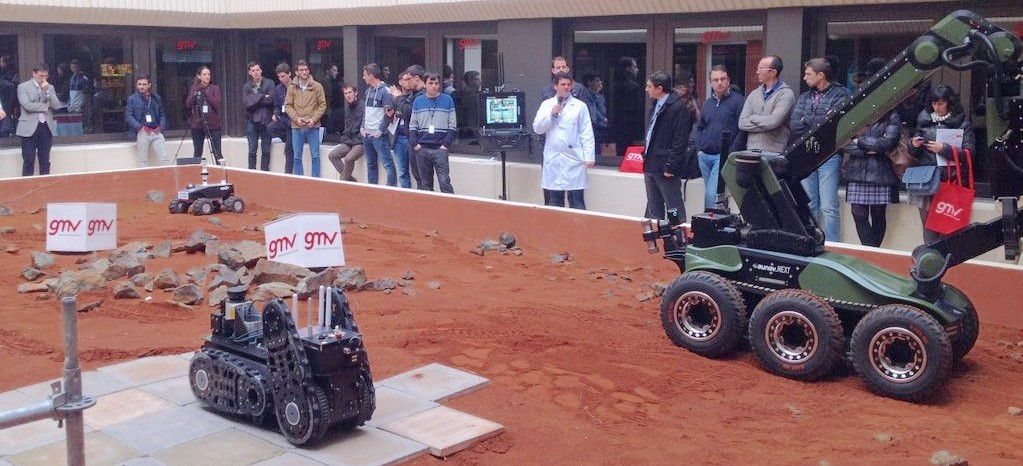
\includegraphics[width=0.8\linewidth]{fotos/2015_V_JornadaRobotica_GMV}}
\caption*{
Demostración de los robots Foxiris de GMV (izquierda), MiR100 de Robotplus (al fondo) y Aunav de Proytecsa (derecha).
}
\end{figure}

Además participamos en el concurso ``Concurrent Design Facility (CDF) for Robotics'' en el que se nos asignó la tarea de diseñar un robot para la monitorización de plantas oil \& gas en menos de tres horas. Obtuvimos el primer premio junto con estudiantes de la UPM.


\begin{figure}[hbtp]
\centerline{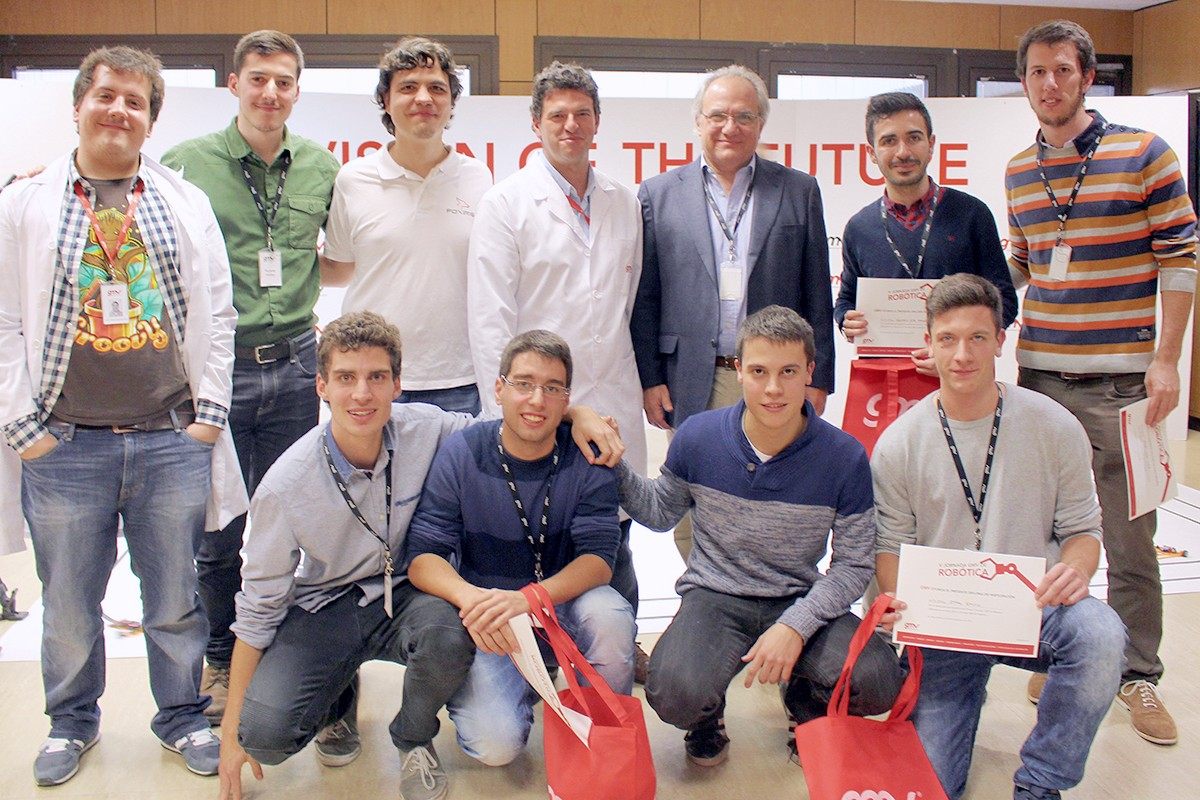
\includegraphics[width=0.8\linewidth]{fotos/2015_V_JornadaRobotica_GMV_team}}
\caption*{
Participantes en el concurso ``Concurrent Design Facility (CDF) for Robotics''. \\
Fila superior: Carlos Crespo (GMV), Carlos García (CRM-UAM), Sergio Martini (GMV), Alberto Medina (GMV), Pedro Hernández (Repsol), Gonzalo Díaz (UPM) y Víctor Uceda (CRM-UAM)
Fila inferior: Luis Paarup, David Matilla, Javier Fernández, Stefan y Pablo Rodríguez -ausente en la foto- (todos de la UPM)
}
\end{figure}






\chapter{Junta directiva actualizada}

La Asociación Club de Robótica-Mecatrónica cuenta con la siguiente junta directiva para el curso 2015-16:

\begin{itemize}
\item Presidente: \textbf{x} ( *)
\item Vice-presidente: \textbf{x} ( *)
\item Secretario: \textbf{x} ( *)
\item Tesorero: \textbf{x} ( *)
\item Vocales: \textbf{x} ( *)
\end{itemize}

* \textit{correos electrónicos @estudiante.uam.es}

En la página web de la asociación está disponible toda la información sobre las juntas directivas de años anteriores:
\url{http://crm.ii.uam.es/historia}


\end{document}
